% =====================================================================
% Manuscript ECOMOD v42 (research-article rewrite of v41)
% How aggregation can conceal composition: aggregate biocapacity and the
% identifiability of modelled ecological-capital drawdown
% Author: Amin Abaee (Independent Researcher, Tehran, Iran)
%
% v42 (2026-10-14): full restructuring into a research article (Introduction
% with questions and contributions -> Methods -> Results organised around three
% propositions and the measured NFA decomposition -> Discussion -> Conclusions).
% Content moved to the Supplementary Information: full symbol table, proofs,
% numerics and verification protocol, extended result tables (b_f sweep,
% drawdown-depth ladder, recovery metric, gate-sign phase dependence), empirical
% details (vintages, alpha-robustness, level fallback, observation-operator
% hierarchy, regeneration anchors), policy extensions, one-stock comparator.
% New in v42: Figure 3 (model dynamics, regenerated from the deposited code),
% the affine-closure derivation of the constant leading eigenvalue, the
% continuous drawdown-depth result, the bounded (not unbounded) debt statement
% with the crossover deficit S^dagger, and the restoration-inertness check.
% All numbers are either carried over verbatim from v41 or regenerated from
% model_sims/twoland_fixed.py at the baseline registry (see CHANGELOG_v41_to_v42).
% Compiles with pdfLaTeX / XeLaTeX / LuaLaTeX / tectonic (elsarticle class).
% =====================================================================
\documentclass[preprint,12pt,authoryear]{elsarticle}

\usepackage{amsmath,amssymb,amsthm}
\usepackage{booktabs}
\usepackage{array}
\usepackage{tabularx}
\usepackage{graphicx}
\graphicspath{{./}{figures/}{manuscript_ECOMOD_v42_src/}{manuscript_ECOMOD_v42_src/figures/}}
\usepackage{enumitem}
\usepackage[colorlinks=true,urlcolor=blue,linkcolor=blue,citecolor=blue]{hyperref}
\emergencystretch=3em
\setlength{\tolerance}{2000}

\newtheorem{proposition}{Proposition}
\newtheorem{corollary}{Corollary}
\newcommand{\pos}[1]{\left[#1\right]_+}
\newcommand{\dconv}{\Delta b_{\mathrm{conv}}}
\newcommand{\Ups}{\Upsilon_c}
\newcommand{\Eceil}{E_{\mathrm{ceil}}}
\newcommand{\Acmin}{A_c^{\min}}
\newcommand{\tconv}{\tau_{\mathrm{conv}}}

\journal{Ecological Modelling}

\begin{document}

\begin{frontmatter}

\title{How aggregation can conceal composition: aggregate biocapacity and the identifiability of modelled ecological-capital drawdown}

\author[1]{Amin Abaee\corref{cor1}}
\ead{amin_abaee@ut.ac.ir}
\cortext[cor1]{Corresponding author. ORCID: 0000-0002-0019-1842.}
\affiliation[1]{organization={Independent Researcher}, city={Tehran}, country={Iran}}

\begin{abstract}
Total biocapacity, the headline index of annual bioproductive supply, is a single number assembled from heterogeneous land accounts whose yields and regeneration rates differ by an order of magnitude. We ask what such an aggregate can and cannot reveal about the land it summarises. We formulate a minimal two-land delay-differential model in which demand in excess of the harvestable flow converts ecological-capital land into fast-provisioning land, with area conserved one-to-one, capital quality carried as a separate state, and degradation acting through an accumulated ecological debt. Three results are proved and verified numerically. (i) Conversion raises the measured aggregate while the capital book falls whenever the fast-land yield exceeds the per-hectare value of capital land (a composition mask), and the aggregate alone cannot distinguish this from genuine growth: with only the total, the capital loss is unidentified. (ii) Under frozen demand the balance point is unique and the capital book is driven to its viability floor above a demand ceiling ($\Eceil\approx1.14$ at the baseline); because the deficit-side dynamics are affine, the leading eigenvalue ($-0.054\,\mathrm{yr}^{-1}$) is constant along the branch, so the drawdown is a floor collision without a fold, without hysteresis and without critical slowing down; with endogenous demand the drawdown depth is a continuous function of initial demand. (iii) The mask is bounded: technology lifts the fast yield by at most a fixed factor, whereas debt erosion is limited only by the sustained deficit. Applied to the National Footprint and Biocapacity Accounts (1961--2022), an exact Divisia decomposition shows that aggregate biocapacity grew $+23\%$ while cropland biocapacity grew $2.85\times$ and the non-cropland book was flat, and per-capita biocapacity halved. The results motivate component reporting alongside any aggregate biocapacity total.
\end{abstract}

\begin{keyword}
biocapacity \sep ecological footprint \sep land-use conversion \sep aggregation \sep identifiability \sep critical slowing down \sep delay differential equations \sep carrying capacity
\end{keyword}

\end{frontmatter}

\section{Introduction}\label{sec:intro}

Carrying capacity is one of ecology's most enduring and most elusive ideas. In classical population biology it is a fixed ceiling; imported into global human ecology it is usually treated as a static boundary, the maximum number of people the Earth can support \citep[cf.][]{Cohen1995}. Treating the ceiling as fixed overlooks a feedback that matters: a population that overshoots its resource base degrades the base and lowers the future ceiling. This paper is concerned with a subtler failure than a fixed ceiling. It concerns the \emph{measurement} on which monitoring and policy depend.

The standard aggregate measure of annual regenerative supply is biocapacity, expressed in the National Footprint and Biocapacity Accounts (NFA) in global hectares (gha). A global hectare is already a value-weighted product of bioproductive area, a yield factor and an equivalence factor \citep{Borucke2013,Lin2018}. Because the weighting sits \emph{inside} the unit, an aggregate biocapacity series does not tell a monitor whether capacity rose because land became more productive, because more land was brought into provision, or because ecological capital was converted into provisioning land. The composite-indicator literature warns that additive aggregation turns weights into trade-offs, so that a deficit in one dimension can be offset by a surplus in another \citep{Nardo2008,Becker2017,Fischer2022}; biocapacity is exactly such a composite, and the footprint framework has been criticised on related grounds \citep{Blomqvist2013,GiampietroSaltelli2014,vdBerghGrazi2015,Galli2016}. The aggregate remains useful as a headline, but only if its components are reported alongside it. What has been missing is a dynamical account of \emph{how} a rising aggregate and a falling capital base can coexist, for how long, and what would be needed to tell them apart.

Coupled human--environment models have largely treated the environment as a single stock or a single aggregate balance: the World3 system \citep{Meadows1972,Meadows1974,Meadows2004}, the Ricardo--Malthus models of Easter Island \citep{BranderTaylor1998,Anderies2000}, and more recent bidirectionally coupled Earth-system frameworks \citep{Motesharrei2016,Donges2017,CalvinBondLamberty2018,HendersonLoreau2018}. Estimates of Earth's carrying capacity span several orders of magnitude \citep{Cohen1995,vdBerghRietveld2004}, some authors reject the notion for humans altogether \citep{Simon1996}, and others let the ceiling itself vary logistically \citep{Meyer1994,MeyerAusubel1999} or treat natural capital as a depreciating asset \citep{Dasgupta2021}. Demographic projections used in most global assessments assume that population unfolds independently of environmental constraints \citep{UN2022}. Within this literature the environment has one book; the question of what an aggregate over two books with different yields and regeneration times can conceal has not been posed as a modelling problem, although the land-use literature has documented the historical operator -- conversion of forest, grassland and wetland into cropland -- in detail \citep{Haberl2007,Krausmann2013,Erb2017}.

Consider an orchard with two kinds of ground. Fast provisioning land -- cropland and intensively managed systems -- yields much and is quickly restored, but has little standing regenerative value. Ecological-capital land -- forest, soil, wetland, long-rotation systems -- has a large standing value and a regenerative flow that is slowly rebuilt. Demand is met first from the fast flow; only the excess converts capital land into provision. Because the aggregate harvest is a value-weighted sum over the two books, conversion can raise the total while the capital book shrinks. A harvest that looks stable, or a rising aggregate measure of capacity, can therefore mask a shrinking ecological-capital account. Neither the orchard nor its harvesters respond instantly -- forest loss, soil degradation and demographic adjustment unfold over decades -- which is why societies can prosper for long periods while quietly undermining their productive base, only to decline abruptly \citep{Tainter1988,Diamond2005}. The companion ledger work calls the general phenomenon the \emph{productivity illusion} \citep{Abaee2026c}; the specific form addressed here is the \emph{composition} illusion, in which the aggregate rises not because technology outpaces degradation but because the books are re-weighted.

We address three questions. \textbf{(Q1)} Under what conditions does conversion of ecological-capital land raise the aggregate while the capital book falls, how long does the mask last, and can the composition be identified from the aggregate? \textbf{(Q2)} Is the resulting capital drawdown a catastrophic shift in the sense of the alternative-stable-states literature \citep{Scheffer2001}, with a fold, hysteresis and early-warning signals, or something structurally different? \textbf{(Q3)} Is the mask self-limiting, and what does recovery require?

The paper makes four contributions. First, it formulates a minimal two-land model (Section~\ref{sec:model}) in which area is conserved one-to-one across three land books, per-hectare capital quality is a separate state, conversion is a rate with an explicit time constant, and degradation acts on the surviving yield through an accumulated ecological debt; the model is a delay differential equation with ecological (regeneration) and demographic delays \citep{Kuang1993,Hutchinson1948}. Second, it proves three propositions (Section~\ref{sec:results}): a composition identity that gives the exact condition for the mask and shows that the aggregate does not identify the capital loss (Proposition~\ref{prop:mask}); the uniqueness of the frozen-demand balance point, the location of the demand ceiling, and the absence of a fold and of critical slowing down, derived from the affine structure of the deficit-side dynamics (Proposition~\ref{prop:ceiling}); and a boundedness asymmetry between the technology and debt channels that makes the mask transient (Proposition~\ref{prop:bounded}). Third, it applies the composition identity to the measured NFA series for 1961--2022 with an exact logarithmic-mean (Divisia) decomposition and the measured land-type accounts (Section~\ref{sec:empirical}). Fourth, it states the falsifiable content of the model as five predictions and draws the reporting implication for sustainability indicators (Sections~\ref{sec:predictions} and \ref{sec:discussion}). The model is deliberately simple and most of its parameters are representative rather than fitted; it is not a forecast. Its purpose is to make the composition logic of aggregate biocapacity explicit and to state which outcomes are structural and which are conditional on effective parameters that are not separately identified.

\section{Methods}\label{sec:model}

\subsection{A two-land model with conserved area and a separate quality state}\label{sec:equations}

The bioproductive area $A_{tot}$ is divided into three books: fast-provisioning land $A_f$ (cropland and intensively managed systems), ecological-capital land $A_c$ (forest, soil, wetland and long-rotation systems, consolidated into one effective class), and a reserve $A_r$ (fallow, retired or not yet allocated land), with $A_f+A_c+A_r=A_{tot}$ at all times. Capital land carries a per-hectare quality index $q\in[0,q_{\max}]$ (a capacity state, not an area), which regenerates logistically,
\begin{equation}\label{eq:Gc}
G_c(q)=\rho_c\,q\left(1-\frac{q}{q_{\max}}\right),
\end{equation}
so that the per-hectare value of capital land, in flow units, is
\begin{equation}\label{eq:Ups}
\Ups(q)=b_c+b_{G,c}\,G_c(q),
\end{equation}
the sum of a direct yield $b_c$ and the value $b_{G,c}$ of the regenerative growth $G_c(q)$. Biocapacity is the additive two-book aggregate
\begin{equation}\label{eq:B}
B=Y_f+Y_c=b_f A_f+\Ups(q)\,A_c ,
\end{equation}
in gha\,yr$^{-1}$. Demand is the footprint $E=eP$ of a population $P$ with constant per-capita footprint $e$, and the shortfall above the human-available flow is
\begin{equation}\label{eq:S}
S=\pos{E-\sigma_f Y_f-\sigma_c Y_c},
\end{equation}
with $\pos{x}=\max(x,0)$ exact (never smoothed) and $\sigma_f=\sigma_c=1$ in the baseline. The shortfall is closed by converting capital land into fast land at a finite rate,
\begin{equation}\label{eq:uc}
u_c=\frac{1}{\tconv}\min\!\left(\frac{S}{b_f},\;A_c-\Acmin\right)\qquad[\mathrm{ha\,yr^{-1}}],
\end{equation}
where $S/b_f$ is the area that would close the shortfall at the fast-land yield, $\Acmin$ is a typed viability floor, and $\tconv$ is the conversion time constant. The land books evolve by one-to-one area transfers only,
\begin{align}
\dot A_c&=-u_c+R_{rc},\label{eq:Ac}\\
\dot A_f&=u_c+\mu A_r-\eta_f A_f,\label{eq:Af}\\
\dot A_r&=-\mu A_r+\eta_f A_f-R_{rc},\label{eq:Ar}
\end{align}
where $\mu A_r$ is cropland maintenance (replanting from the reserve), $\eta_f A_f$ is fast-land retirement to the reserve, and $R_{rc}$ is an explicit, surplus-gated restoration flow from reserve to capital land,
\begin{equation}\label{eq:Rrc}
R_{rc}=\chi_r\,A_r\,\pos{B-E},
\end{equation}
which is the only route back into the capital book. Equations \eqref{eq:Ac}--\eqref{eq:Ar} sum to zero, so the reserve is a constrained balance rather than an independent state. Quality regenerates with a recruitment delay, population follows a delayed logistic law \citep{Pearl1925,Hutchinson1948} on the carrying capacity $K=B/e$, and degradation acts on the surviving fast-land yield through an accumulated ecological debt $D$:
\begin{align}
\dot q&=G_c\big(q(t-\tau_g)\big),\label{eq:q}\\
\dot P&=rP\left(1-\frac{P}{K(t-\tau_p)}\right),\qquad K=\max(B/e,\,K_{\min}),\label{eq:P}\\
b_f&=\big(b_{f0}+T_b(t)\big)\,e^{-\alpha D},\label{eq:bf}\\
\dot D&=\pos{E-B}-\eta D,\label{eq:D}\\
T_b(t)&=\frac{\Delta b}{1+e^{-\kappa_w(t-t_{wave})}}.\label{eq:Tb}
\end{align}
The technology wave $T_b$ is a bounded logistic yield step (off unless stated). The state is $(A_f,A_c,q,P,D)$ with one delay each in regeneration and demography; a timber-liquidation channel and a direct fast-to-capital restoration flow are stated extensions that are off in every reported run (Supplementary Information, SI~\S S1).

Five conventions are essential. (i) \emph{The positive part is exact.} A smoothed ramp would leak conversion when $E<B$; the one-sided deficit mechanism is the model's content, so $\pos{\cdot}$ is never regularised and stability at $S=0$ is one-sided. (ii) \emph{Conversion is a rate.} $S/b_f$ is a stock (ha); it becomes a rate only through $\tconv$, so $u_c$ is dimensionally ha\,yr$^{-1}$ and conversion is never instantaneous. (iii) \emph{Area is conserved one-to-one and capacity is a separate book.} Every area flow in \eqref{eq:Ac}--\eqref{eq:Ar} moves hectares between books; regeneration $G_c$ is a flow of capacity into $q$ and never transfers land, so conservation is a property of the equations, not an identity imposed afterwards. (iv) \emph{Flows and stocks are never interchanged.} $B$ and $E$ are annual flows (gha\,yr$^{-1}$); $D$ is the accumulation of a flow (gha) repaid at rate $\eta$; $b_f,b_c$ are flow yields and $b_{G,c}$ is a standing value. (v) \emph{A sustainable cropland equilibrium exists.} Because \eqref{eq:Af} contains the maintenance term $\mu A_r$, a positive fast book $A_f^*$ is sustained without conversion; without it the fast book would decay to zero at every equilibrium.

Two positive feedback loops act on different books. The \emph{conversion loop} reallocates area: $A_c\downarrow\to A_f\uparrow\to B\uparrow$ (if $b_f>\Ups$) $\to K\uparrow\to P\uparrow\to S\uparrow\to A_c\downarrow$; it raises the aggregate while the capital book falls and is the composition mechanism of this paper. The \emph{debt loop} erodes the surviving yield: $D\uparrow\to b_f\downarrow\to B\downarrow\to S\uparrow\to D\uparrow$; it later turns against the aggregate and is one reason the mask is bounded (Proposition~\ref{prop:bounded}).

\subsection{Parameters and their status}\label{sec:params}

Table~\ref{tab:params} lists the baseline registry. The capital book is a strategic reduction: real ecological capital is a vector of land types with their own yields, values and regeneration times, and the two-book model treats them as one effective class. Consequently most parameters are representative, effective quantities rather than estimates, and the results are stated with that status attached. Two quantities are empirically anchored: the capital-land regeneration timescale, which we bound from raw recovery curves in two ecosystem classes (secondary forest, \citealp{Poorter2016}; collapsed fish stocks, RAM Legacy, cf.\ \citealp{HutchingsReynolds2004,Neubauer2013}; with soil organic carbon, \citealp{Poeplau2011}, between them; SI~\S S5.5), and the provisioning-book yield and area, which we calibrate against NFA cropland biocapacity and the FAO crop-yield index (SI~\S S5.3). The regeneration anchors bound a \emph{band} of effective timescales ($\approx$25--33\,yr, representative $\approx$29\,yr; forest $t_{50}\approx30$\,yr, fishery $t_{50}\approx5.6$\,yr) and are statements about the regeneration rate, not the lag $\tau_g$; the two are kept distinct throughout. The baseline sits in the composition-premium regime, $\dconv=b_f-\Ups(q)>0$, which is the regime in which the mask is possible (Section~\ref{sec:mask}); Table~\ref{tab:params} therefore fixes a regime, not a prediction.

\begin{table}[!htbp]
\centering\footnotesize
\caption{Baseline parameter registry (single source of truth for all reported runs) and the status of each parameter. ``Representative'' values are effective, lumped quantities that are not individually identified; ``anchored'' values are bounded by independent data (SI~\S S5); ``extension'' parameters are stated but off in the base model. Full symbol table with units in SI~\S S1.}
\label{tab:params}
\setlength{\tabcolsep}{4pt}
\begin{tabularx}{\textwidth}{@{}>{\raggedright\arraybackslash}p{0.13\textwidth} >{\raggedright\arraybackslash}p{0.2\textwidth} >{\raggedright\arraybackslash}X >{\raggedright\arraybackslash}p{0.26\textwidth}@{}}
\toprule
Parameter & Value & Meaning & Status \\
\midrule
$\rho_c$ & $0.08$\,yr$^{-1}$ & quality regeneration rate of capital land & representative; timescale band anchored \\
$b_{f0}$ & $0.85$\,gha\,ha$^{-1}$\,yr$^{-1}$ & base fast-land flow yield & representative (NFA cropland book $\approx0.93$ in 1961) \\
$b_c$ & $0.05$\,gha\,ha$^{-1}$\,yr$^{-1}$ & capital-land direct yield & representative \\
$b_{G,c}$ & $0.8$\,gha\,ha$^{-1}$ & standing value of one hectare of capital & representative \\
$q_{\max}$ & $1.0$ & quality ceiling & normalisation \\
$\mu$ & $0.06$\,yr$^{-1}$ & cropland maintenance (reserve$\to$fast) & representative \\
$\eta_f$ & $0.05$\,yr$^{-1}$ & fast-land retirement (fast$\to$reserve) & representative \\
$\tconv$ & $1.0$\,yr & conversion time constant & representative \\
$\alpha$ & $0.03$\,gha$^{-1}$ & degradation of $b_f$ per unit debt & representative \\
$\eta$ & $0.05$\,yr$^{-1}$ & debt-repayment rate ($>0$) & representative \\
$e$ & $0.55$\,gha\,cap$^{-1}$\,yr$^{-1}$ & per-capita footprint (constant) & representative \\
$r$ & $0.02$\,yr$^{-1}$ & intrinsic population growth & representative \\
$\tau_g,\ \tau_p$ & $20,\ 25$\,yr & regeneration and demographic delays & representative; $\tau_p$ lumps institutional lags \\
$A_{tot}$ & $2.5$\,ha & total bioproductive area & normalisation \\
$\sigma_f,\ \sigma_c$ & $1,\ 1$ & human-available flow shares & baseline ($<1$: reservation extension) \\
$\chi_r$ & $0.10$\,gha$^{-1}$ & surplus-gated restoration coefficient & on with endogenous demand; off under frozen demand \\
$\Acmin$, $A_r^{\min}$,\newline $K_{\min}$ & $0.05$\,ha, $0.10$\,ha,\newline $0.02$\,cap & typed floors & domain constraints \\
$\Delta b$, $\kappa_w$,\newline $t_{wave}$ & $1.0$, $0.1$\,yr$^{-1}$,\newline $40$\,yr & technology wave & extension; off in all reported runs \\
\bottomrule
\end{tabularx}
\end{table}

\subsection{Data and the observation operator}\label{sec:data}

The empirical analysis uses the world series of the National Footprint and Biocapacity Accounts (2025 edition): the aggregate biocapacity and footprint series for 1961--2022, and the land-type biocapacity matrix (cropland, grazing land, forest products, fishing grounds, built-up land). The land-type vintage incorporates a retroactive re-basing and gives a slightly higher aggregate growth ($+24.5\%$, $\Delta\ln B=+0.219$) than the aggregate series ($+23.0\%$, $\Delta\ln B=+0.207$); rather than blend the vintages we report the attribution across both (SI~\S S5.2). Population is from the same accounts. The independent proxies that advance past the aggregate are FAOSTAT cropland area (arable plus permanent crops) for $A_f$ and a normalised FAO crop-yield index for $b_f$, calibrated at the base year either by a nominal cropland share $\alpha$ of 1961 biocapacity or directly against measured NFA cropland biocapacity \citep{FAO2023}; forest area \citep{FAO2020}, historical land-use reconstructions \citep{Hurtt2011,KleinGoldewijk2017}, remote-sensing land cover \citep{ESA2017,Copernicus2019} and cropland-productivity maps \citep{Monfreda2008} form the hierarchy of extensions described in SI~\S S5.4.

The decomposition instrument is the exact logarithmic-mean (Divisia) identity. Writing $B_t=X_t+C_t$ with a proxy fast-book component $X_t=\hat b_{f,t}A_{f,t}$ and residual $C_t=B_t-X_t$,
\begin{equation}\label{eq:divisia}
\begin{split}
\Delta\ln B&=w_X\big(\Delta\ln b_f+\Delta\ln A_f\big)+w_C\,\Delta\ln C,\\
w_X&=\frac{L(X_T,X_0)}{L(B_T,B_0)},\qquad w_C=\frac{L(C_T,C_0)}{L(B_T,B_0)},
\end{split}
\end{equation}
with the logarithmic mean $L(a,b)=(a-b)/(\ln a-\ln b)$ for $a\neq b$ and $L(a,a)=a$. The identity holds exactly whenever $X$ and $C$ are positive at both endpoints; average-share weights do not (they overshoot by $\approx11\%$ here), and the level decomposition $\Delta B=\Delta X+\Delta C$ is the exact fallback when the residual is not positive (SI~\S S5.2). The extensive/intensive split uses the exact identity $d\ln B=d\ln(B/P)+d\ln P$.

\subsection{Numerical solution and verification}\label{sec:numerics}

The delay system is integrated by the method of steps with an explicit first-order scheme ($\Delta t=0.05$\,yr for the demonstration run, $0.1$ and $0.05$\,yr for the drawdown sweeps), the exact positive part, clamps enforcing $A_c\ge\Acmin$, $A_f\ge0$, $q\in[0,q_{\max}]$, $K\ge K_{\min}$, and delay histories populated with the initial state rather than zero (a zero history produces spurious early collapses). Area conservation is verified at every step ($\max|A_f+A_c+A_r-A_{tot}|=2.2\times10^{-16}$). Every analytic quantity below (balance points, ceiling, eigenvalues, composition diagnostic) is recomputed from the deposited code and asserted against the stated value before a figure is written. Drawdown thresholds are reported as bands because the operational floor-contact criterion depends on the tolerance and step size (Section~\ref{sec:ceiling}). The deposited solver evaluates the regeneration term of \eqref{eq:q} at the current rather than the delayed quality; because $q$ is monotone and the regenerative term is small at the baseline ($b_{G,c}G_c\le0.016$ against $b_c=0.05$), applying the delay changes the reported quantities by less than $1\%$ (window $149$ vs.\ $150$\,yr; thresholds within $0.001$), and both variants are reported in SI~\S S3. Code and data are deposited (Zenodo record 22554480).

\section{Results}\label{sec:results}

\subsection{The composition mask and what the aggregate cannot identify}\label{sec:mask}

The per-hectare value of capital land $\Ups(q)$ is a concave quadratic in $q$ with an interior maximum at $q^*=q_{\max}/2$, where $\Ups(q^*)=b_c+b_{G,c}\rho_c q_{\max}/4=0.066$ at the baseline; the regenerative term there ($0.016$) is about one third of the direct yield ($0.05$; ratio $0.32$), so capital value is only modestly enhanced by regeneration. The quantity that governs what conversion does to the aggregate is the \emph{composition diagnostic}
\begin{equation}\label{eq:dconv}
\dconv(q,D)=b_f(D)-\Ups(q),
\end{equation}
the difference between what a hectare yields in the fast book and what it is worth in the capital book. At the baseline $\dconv=+0.787,\ +0.784,\ +0.794$ at $q=0.3,\,0.6,\,0.9$: the model sits robustly in the composition-premium regime, in which converting a hectare raises current accounting capacity. The three regimes $\dconv>0$ (premium: conversion raises $B$, mask possible), $\dconv=0$ (first-order neutrality, non-generic) and $\dconv<0$ (discount: conversion lowers $B$ at once, no mask) are the only shape distinction the quality-based model admits; because $Y_c$ is linear in $A_c$ at fixed $q$, there is no area-based capacity maximum and no regime split of the kind an area-based regeneration law would produce.

\begin{proposition}[Composition identity, mask and non-identifiability]\label{prop:mask}
Let $T_b\equiv0$, $R_{rc}\equiv0$ and hold $D$ fixed, so that $b_f$ is constant. Along any solution of \eqref{eq:B}--\eqref{eq:q},
\begin{equation}\label{eq:identity}
\dot B=\dconv(q)\,u_c+b_f\big(\mu A_r-\eta_f A_f\big)+b_{G,c}\,G_c'(q)\,A_c\,\dot q .
\end{equation}
\begin{enumerate}[label=(\roman*)]
\item On any interval on which $u_c>0$, $\dot A_c<0$, and the conversion contribution to $\dot B$ is positive if and only if $\dconv(q)>0$. In the pure-conversion subsystem ($\mu A_r=\eta_f A_f$, $q=q_{\max}$), $\dot B>0\iff\dconv>0$ whenever $u_c>0$: the aggregate rises while the capital book falls.
\item Under frozen demand $E$ and $\dconv>0$, the shortfall $S$ is strictly decreasing along pure conversion ($\dot S=-\dot B<0$ on $S>0$), so the mask is a transient: the trajectory converges to a state with $S=0$ (the balance point of Proposition~\ref{prop:ceiling}) or with $A_c=\Acmin$.
\item The aggregate \eqref{eq:B} is one linear functional of the two areas. From the series $B(t)$ alone, any observed change $\Delta B\ge0$ is consistent with every capital change $\Delta A_c\in[\Acmin-A_c(0),\,0]$ (the fast-book change $\Delta A_f=(\Delta B-\Ups\Delta A_c)/b_f$ absorbs the difference); the capital loss is unidentified. If $b_f$ and $A_f$ are observed independently, the residual $C=B-b_fA_f=\Ups(q)A_c$ identifies the product $\Ups(q)A_c$, but $b_c$, $b_{G,c}$, $\rho_c$ and $q$ enter only through $\Ups=b_c+b_{G,c}\rho_c q(1-q/q_{\max})$ and are not separately identifiable from $C$; the identifiable combinations are $\Ups$ (equivalently $b_{c,\mathrm{eff}}$) and $b_{G,c}\rho_c$.
\end{enumerate}
\end{proposition}

\begin{proof}
Differentiate \eqref{eq:B} with $b_f$ constant and substitute \eqref{eq:Ac}--\eqref{eq:Af} with $R_{rc}=0$: $\dot B=b_f(u_c+\mu A_r-\eta_fA_f)-\Ups u_c+b_{G,c}G_c'(q)A_c\dot q$, which is \eqref{eq:identity}. (i) is immediate from \eqref{eq:identity} and $\dot A_c=-u_c$. (ii) With $\sigma_f=\sigma_c=1$ and $S>0$, $S=E-B$, so $\dot S=-\dot B=-\dconv u_c<0$; $S$ is bounded below by zero and $A_c$ is non-increasing and bounded below by $\Acmin$, so the trajectory converges to a state with $S=0$ or $A_c=\Acmin$. (iii) is the statement that a single linear equation in two unknowns has a one-parameter family of solutions, and that $\Ups$ depends on $(b_c,b_{G,c},\rho_c,q)$ only through the stated combination.
\end{proof}

Figure~\ref{fig:model}a shows the mask at the baseline under frozen demand $E=0.825$ (restoration off, $A_{f0}=0.6$, $A_{c0}=1.5$, $q_0=0.9$, $A_r(0)=0.4$). Biocapacity rises from $0.594$ to $0.825$ ($+39\%$) while capital land falls from $1.500$ to $0.808$ ($-46\%$) and fast land rises from $0.600$ to $0.923$; quality rises from $0.9$ to $1.0$, so the capital \emph{quality} is not drawn down even as its \emph{area} is. The area changes are one-to-one ($\Delta A_f+\Delta A_c+\Delta A_r=0$ to machine precision). The dynamics are fast at first and then asymptotic: because the deficit-side land subsystem is affine (Proposition~\ref{prop:ceiling}(ii)), the approach to the balance point is exponential at the slow rate $|\lambda_1|=0.054\,\mathrm{yr}^{-1}$ (e-folding $\approx19$\,yr), so within $25$\,yr $98\%$ of the rise in $B$ and $85\%$ of the fall in $A_c$ have occurred ($B=0.820$, $A_c=0.913$; $97\%$ of the fall by $50$\,yr), while the strict inequalities $\dot B>0$ and $\dot A_c<0$ persist for $\approx150$\,yr at numerical resolution. The slow tail is reserve equilibration: retirement of fast land to the reserve lowers the fast flow, re-opens a small shortfall, and converts a little more capital, until the reserve reaches its equilibrium share $A_r/A_f=\eta_f/\mu$. The window is therefore not a fixed horizon: its scale is set by $\lambda_1$, which depends on $\tconv$, $\mu$, $\eta_f$ and the yield ratio $b_c/b_f$ (SI~\S S2.2), and its amplitude by $\dconv$ and the initial deficit.

Two consequences of Proposition~\ref{prop:mask}(iii) frame the empirical analysis of Section~\ref{sec:empirical}. First, the composition signature ($B$ rises while $A_c$ falls) is contemporaneously observable only in the two-book series; a monitor who sees the aggregate alone cannot distinguish a composition mask from broad growth. Second, independent proxies for the fast book ($A_f$, $b_f$) convert the aggregate into a measured fast book and a residual, which is the most that can be identified without independent ecological valuation of the capital book. We refer to the two readings as the \emph{composition mask} ($B$ rises while $A_c$ falls; requires $\dconv>0$) and the \emph{liquidation mask} ($E$ steady while $A_c$ falls; requires nothing); which of the two holds is itself a discriminating observable.

\begin{figure}[!htbp]
\centering
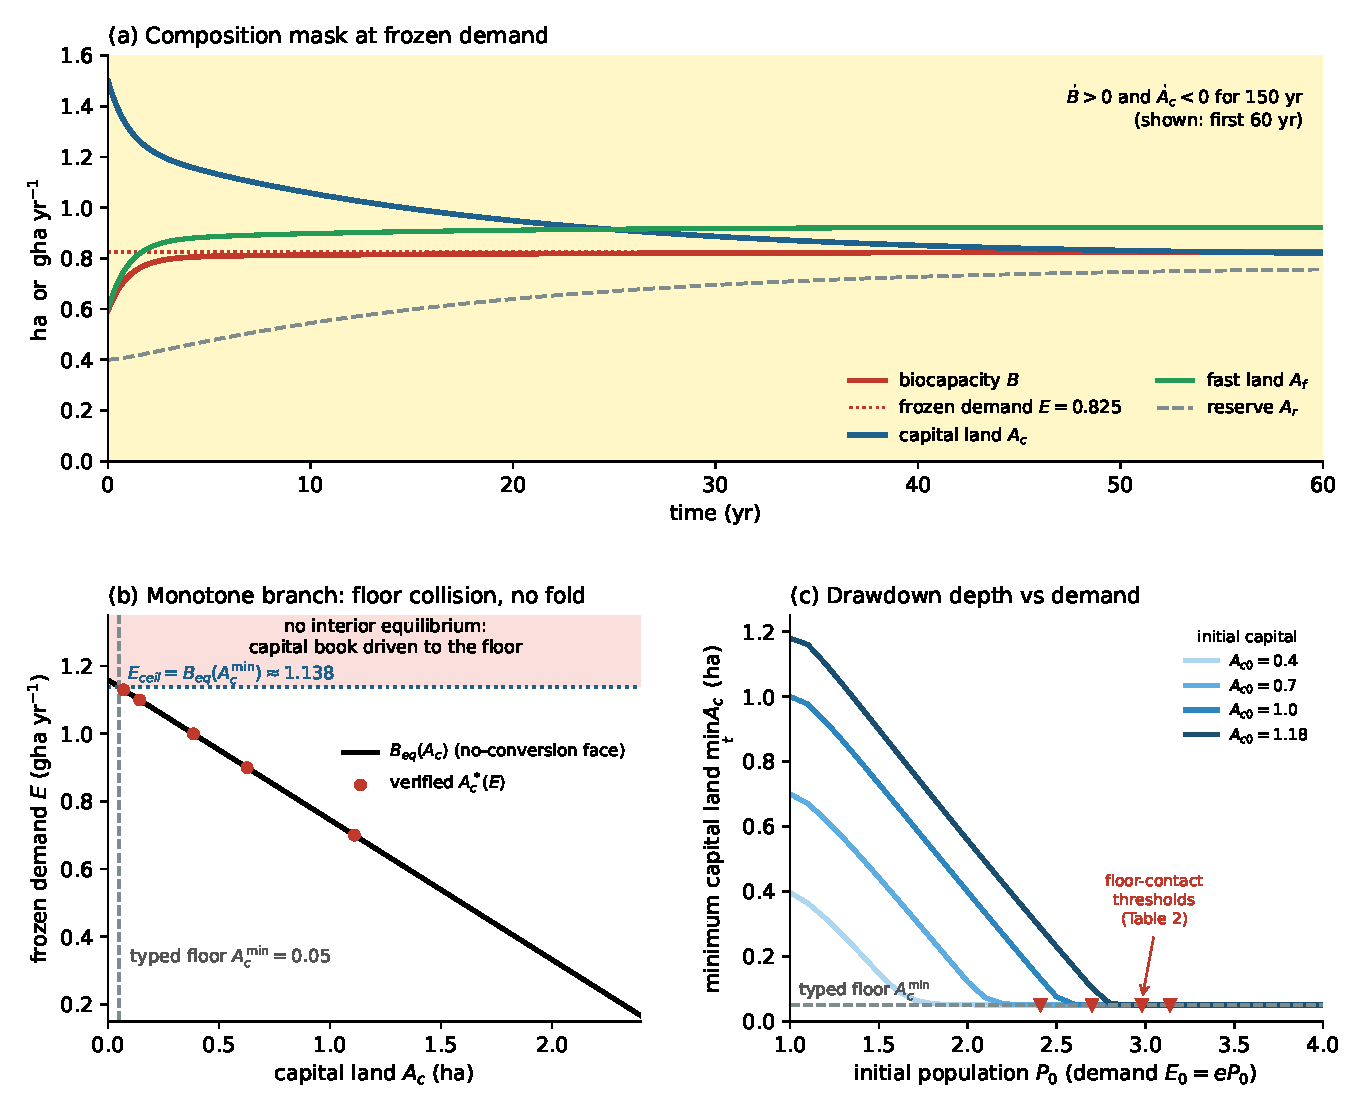
\includegraphics[width=\textwidth]{fig1_model_dynamics}
\caption{Model dynamics at the baseline registry (Table~\ref{tab:params}), regenerated from the deposited code. (a) Composition mask under frozen demand $E=0.825$ (restoration off, $A_{f0}=0.6$, $A_{c0}=1.5$, $q_0=0.9$): biocapacity $B$ rises from $0.594$ to $0.825$ while capital land $A_c$ falls from $1.500$ to $0.808$ and fast land $A_f$ rises from $0.600$ to $0.923$; the shaded region marks the interval on which $\dot B>0$ and $\dot A_c<0$ hold simultaneously ($\approx150$\,yr at numerical resolution; only the first 60\,yr are shown; $98\%$ of the rise in $B$ and $85\%$ of the fall in $A_c$ occur within the first 25\,yr). (b) The frozen-demand balance branch $B_{eq}(A_c)$ of Proposition~\ref{prop:ceiling}, strictly decreasing in $A_c$, with the verified balance points $A_c^*(E)=1.110,\,0.626,\,0.385,\,0.143,\,0.070$ at $E=0.70,\,0.90,\,1.00,\,1.10,\,1.13$; the branch meets the typed floor $\Acmin=0.05$ at the demand ceiling $\Eceil\approx1.138$, above which no balance point exists and the capital book is driven to the floor (shaded). (c) Endogenous-demand runs ($\tau_g=20$, $\tau_p=25$\,yr, $\chi_r=0.10$): the minimum capital land reached during a run is a continuous, monotone function of initial demand $P_0$ (hence $E_0=eP_0$) for each initial capital $A_{c0}$; the floor is approached asymptotically, and the floor-contact thresholds of Table~\ref{tab:model} (triangles) are the operational points at which the floor is reached to within $10^{-6}$. There is no discontinuity in the outcome as a function of demand.}
\label{fig:model}
\end{figure}

\subsection{The drawdown is a demand-driven floor collision, not a fold}\label{sec:ceiling}

With endogenous population there is no interior steady state with active conversion: at a demographic equilibrium $P=K=B/e$, so $E=B$ and $S=0$. Conversion is therefore a transient regime, and its steady states exist only under a frozen exogenous demand pinned above the flow. The frozen-demand system is where the question of a catastrophic shift must be posed, and it has a complete answer.

\begin{proposition}[Balance point, demand ceiling and affine deficit-side dynamics]\label{prop:ceiling}
Assume frozen demand $E$, $T_b\equiv0$, $R_{rc}\equiv0$, $q=q_{\max}$ (the attractor of \eqref{eq:q} for $q(0)>0$) and $D=0$. Let $k=\mu/(\mu+\eta_f)$ and
\begin{equation}\label{eq:Beq}
B_{eq}(A_c)=b_{f0}\,k\,(A_{tot}-A_c)+b_cA_c=b_{f0}kA_{tot}-(b_{f0}k-b_c)A_c .
\end{equation}
\begin{enumerate}[label=(\roman*)]
\item Equilibria of the land subsystem on the no-conversion face $S=0$ satisfy $A_f=k(A_{tot}-A_c)$, $A_r=(1-k)(A_{tot}-A_c)$ and $B_{eq}(A_c)\ge E$. If $b_{f0}k>b_c$, $B_{eq}$ is strictly decreasing, so the balance point $B_{eq}(A_c^*)=E$ is unique,
\begin{equation}\label{eq:Acstar}
A_c^*(E)=\frac{b_{f0}kA_{tot}-E}{b_{f0}k-b_c},
\end{equation}
and it lies above the typed floor if and only if $E<\Eceil:=B_{eq}(\Acmin)$.
\item On the deficit side ($S>0$, $S/b_f<A_c-\Acmin$) the land subsystem is affine in $z=(A_f,A_c)$, $\dot z=Jz+c$, with
\begin{equation}\label{eq:J}
J=\begin{pmatrix}-\tconv^{-1}-\mu-\eta_f & -\mu-\dfrac{b_c}{b_f\tconv}\\[8pt] \tconv^{-1} & \dfrac{b_c}{b_f\tconv}\end{pmatrix},
\qquad \det J=\frac{\mu+\eta_f}{\tconv}\Big(k-\frac{b_c}{b_f}\Big),
\end{equation}
and $\operatorname{tr}J<0$.
$J$ does not depend on $E$ or on the state, $\det J>0$ exactly when $B_{eq}$ is decreasing, and the fixed point of the affine system is the balance point of (i). For $E<\Eceil$ the balance point is admissible and every trajectory that remains in this regime converges to it at the constant rates given by the eigenvalues of $J$; for $E>\Eceil$ the fixed point lies below the floor, the trajectory reaches the face $A_c=\Acmin$ and remains there with a persistent shortfall $S^*=E-\Eceil>0$. The ceiling is a collision of the equilibrium with a face of the admissible set, not a bifurcation of the vector field: there is no second branch, no fold, no hysteresis, and the leading eigenvalue does not tend to zero as $E\to\Eceil$.
\item Beyond the ceiling, with degradation active, the debt converges to the unique root $D^*(E)$ of $\eta D=E-B_{eq}(\Acmin;D)$, where $B_{eq}(\cdot\,;D)$ uses $b_{f0}e^{-\alpha D}$, provided $\eta>\alpha b_{f0}k(A_{tot}-\Acmin)$; $D^*$ is increasing in $E$.
\end{enumerate}
\end{proposition}

\begin{proof}
(i) With $S=0$ and $R_{rc}=0$, \eqref{eq:Af} gives $\mu A_r=\eta_fA_f$, hence $A_r/A_f=\eta_f/\mu$ and, with $A_r=A_{tot}-A_f-A_c$, $A_f=k(A_{tot}-A_c)$; substituting into \eqref{eq:B} with $q=q_{\max}$ ($\Ups=b_c$) and $D=0$ gives $B=B_{eq}(A_c)$, and $S=0$ requires $B\ge E$. Strict monotonicity and \eqref{eq:Acstar} follow from $b_{f0}k>b_c$. (ii) On the deficit side $u_c=(E-b_fA_f-b_cA_c)/(b_f\tconv)$ is affine in $z$; substituting into \eqref{eq:Ac}--\eqref{eq:Af} with $A_r=A_{tot}-A_f-A_c$ gives $J$ and a constant vector $c$ by direct differentiation; $\det J$ follows by expansion, and $\operatorname{tr}J=-\tconv^{-1}(1-b_c/b_f)-\mu-\eta_f<0$ for $b_c<b_f$. The fixed point solves $u_c=0$ and $\mu A_r=\eta_fA_f$, i.e.\ it is the balance point. Because $J$ is constant, convergence rates are constant along the branch. (iii) The map $D\mapsto\eta D+B_{eq}(\Acmin;D)-E$ is continuous, negative at $D=0$ when $E>\Eceil$, tends to $+\infty$, and is strictly increasing when $\eta>\alpha b_{f0}k(A_{tot}-\Acmin)\ge-\partial_DB_{eq}$; hence it has a unique root, which increases with $E$.
\end{proof}

At the baseline $k=0.5455$, the slope $b_{f0}k-b_c=0.414$, and $\Eceil=1.138$; the balance points $A_c^*(E)=1.110,\,0.626,\,0.385,\,0.143,\,0.070$ at $E=0.70,\,0.90,\,1.00,\,1.10,\,1.13$ agree with the integrated equilibria (Fig.~\ref{fig:model}b). The eigenvalues of $J$ are real and negative, $\lambda_1=-0.0537$ and $\lambda_2=-0.998\,\mathrm{yr}^{-1}$; $\lambda_1$ varies only weakly with the fast-land yield, from $-0.0522$ at $b_f=0.60$ to $-0.0556$ at $b_f=2.00$ (Table~\ref{tab:model}a), and never changes sign. There is no universal scalar stability index: the conversion-loop gain is the state- and parameter-dependent $\dconv$, of order $1\,\mathrm{gha\,ha^{-1}\,yr^{-1}}$, and the return rate is $|\lambda_1|$ of order $10^{-2}\,\mathrm{yr}^{-1}$. Beyond the ceiling the debt fixed points are $D^*=1.19$ and $5.38$ at $E=1.158$ and $1.238$ (integrated values $1.21$ and $5.39$); the monotonicity condition of (iii) holds with margin ($\alpha b_{f0}k(A_{tot}-\Acmin)=0.034<\eta=0.05$), so under frozen demand the debt saturates rather than running away.

The statement ``no critical slowing down'' is precise here. By critical slowing down we mean that the least-negative eigenvalue of the relevant linearisation tends to $0^-$ as a parameter approaches a fold, so that the return time $T_{ret}\approx-1/\lambda_1$ diverges. In Proposition~\ref{prop:ceiling} the linearisation is constant along the entire branch, so neither $\lambda_1$ nor $T_{ret}\approx19$\,yr changes as $E\to\Eceil$. The only early-warning signal the model offers is a \emph{boundary} signal, the capital book approaching its typed floor, which is observable only in the two-book series.

With endogenous demand the same structure appears as a continuous drawdown. Figure~\ref{fig:model}c shows the minimum capital land reached during a run as a function of initial population $P_0$ for four initial capital stocks: the curves are continuous and monotone, the floor is approached asymptotically (because $u_c\le(A_c-\Acmin)/\tconv$, the distance to the floor decays exponentially during a sustained deficit and is never crossed), and higher initial capital supports higher demand before the floor is reached. The ``collapse thresholds'' of the earlier literature on this model are therefore operational quantities: Table~\ref{tab:model}b reports the initial demand at which the floor is approached to within $10^{-2}$, $10^{-4}$ and $10^{-6}$ of its value. The $10^{-6}$ floor-contact values ($P_0\approx2.41,\,2.70,\,2.98,\,3.14$ for $A_{c0}=0.40,\,0.70,\,1.00,\,1.18$) are the ones a bisection on exact floor contact returns; they rise monotonically with initial capital, as do the looser criteria, and no criterion exhibits a jump. Two robustness checks bear on the predictions of Section~\ref{sec:predictions}: the floor-contact threshold at $A_{c0}=1.0$ is identical to three decimals for $\tau_g=5$, $20$ and $40$\,yr, and identical to three decimals with the restoration coefficient $\chi_r=0.10$ and $\chi_r=0$ (SI~\S S4). The first reflects the small leverage of the regenerative term at the baseline and the monotone quality dynamics; the second reflects the fact that a surplus-gated flow is inert during the shortfall that produces the drawdown.

\begin{table}[!htbp]
\centering\small
\caption{Model results at the baseline registry. (a) Composition diagnostic at $q^*=q_{\max}/2$ ($\Ups(q^*)=0.066$), eigenvalues of the deficit-side matrix $J$ of \eqref{eq:J} and the demand ceiling, for a sweep of the fast-land yield $b_f$ (all other parameters at baseline). (b) Initial demand $P_0$ (initial footprint $E_0=0.55P_0$) at which the minimum capital land reached during an endogenous-demand run ($A_{f0}=0.6$, $q_0=0.9$, $\tau_g=20$, $\tau_p=25$\,yr) comes within the stated distance of the typed floor $\Acmin=0.05$; the first two columns are read from a $P_0$ grid of step $0.1$ ($\Delta t=0.1$\,yr, $T=400$\,yr), the last is a bisection on exact floor contact ($\Delta t=0.05$\,yr, $T=1000$\,yr). Drawdown depth is continuous in $P_0$ (Fig.~\ref{fig:model}c); the thresholds are a band, not a single value.}
\label{tab:model}
\begin{tabular}{l l l l l}
\toprule
\multicolumn{5}{l}{(a) Fast-land yield sweep (all rows composition-premium, $\dconv>0$)}\\
$b_f$ & $\dconv(q^*)$ & $\lambda_1$ (yr$^{-1}$) & $\lambda_2$ (yr$^{-1}$) & $\Eceil$ \\
\midrule
$0.60$ & $+0.534$ & $-0.0522$ & $-0.975$ & $0.804$ \\
$0.85$ (baseline) & $+0.784$ & $-0.0537$ & $-0.998$ & $1.138$ \\
$1.20$ & $+1.134$ & $-0.0547$ & $-1.014$ & $1.606$ \\
$2.00$ & $+1.934$ & $-0.0556$ & $-1.029$ & $2.675$ \\
\bottomrule
\end{tabular}

\medskip
\begin{tabular}{l l l l}
\toprule
\multicolumn{4}{l}{(b) Initial demand $P_0$ at which $\min_tA_c$ approaches $\Acmin$ to within:}\\
$A_{c0}$ (ha) & within $10^{-2}$ & within $10^{-4}$ & floor contact ($10^{-6}$) \\
\midrule
$0.40$ & $\approx1.8$ & $\approx2.1$ & $\approx2.41$ \\
$0.70$ & $\approx2.2$ & $\approx2.4$ & $\approx2.70$ \\
$1.00$ & $\approx2.6$ & $\approx2.8$ & $\approx2.98$ \\
$1.18$ & $\approx2.8$ & $\approx3.0$ & $\approx3.14$ \\
\bottomrule
\end{tabular}
\end{table}

\subsection{The mask is bounded: technology saturates, debt does not}\label{sec:bounded}

Both the technology wave and the degradation act on the same coefficient, the fast-land yield $b_f$ of \eqref{eq:bf}, and they do so multiplicatively. This yields a structural asymmetry.

\begin{proposition}[Boundedness asymmetry]\label{prop:bounded}
Under \eqref{eq:bf}--\eqref{eq:Tb}:
\begin{enumerate}[label=(\roman*)]
\item the technology factor satisfies $1\le(b_{f0}+T_b(t))/b_{f0}\le1+\Delta b/b_{f0}$ for all $t$, so the logarithmic gain of the yield channel is bounded by $\ln(1+\Delta b/b_{f0})$ uniformly in time ($0.78$ at the baseline);
\item the debt satisfies $D(t)\le\max\{D(0),\ \sup_{s\le t}\pos{E-B}(s)/\eta\}$, and $D\to S^*/\eta$ whenever the shortfall settles at $S^*$; the degradation factor $e^{-\alpha D}$ is therefore bounded below only through the sustained shortfall;
\item the degradation loss exceeds the maximal technology gain once the sustained shortfall exceeds $S^\dagger=(\eta/\alpha)\ln(1+\Delta b/b_{f0})$, equal to $1.30\,\mathrm{gha\,yr^{-1}}$ at the baseline.
\end{enumerate}
Under an additive degradation law $b_f=b_{f0}+T_b-\alpha D$ the two channels enter symmetrically and (iii) reduces to a comparison of $\Delta b$ with $\alpha D^*$; the asymmetry is a property of the multiplicative form.
\end{proposition}

\begin{proof}
(i) is $0\le T_b\le\Delta b$. (ii) From \eqref{eq:D}, $\dot D\le\bar S-\eta D$ with $\bar S=\sup_{s\le t}\pos{E-B}$, so $D(t)\le\max\{D(0),\bar S/\eta\}$ by comparison; if $\pos{E-B}\to S^*$ then $D\to S^*/\eta$. (iii) compares $\alpha S^*/\eta$ with $\ln(1+\Delta b/b_{f0})$.
\end{proof}

The proposition corrects a tempting overstatement: debt does not compound without bound under a fixed shortfall -- it saturates at $S^*/\eta$ -- but its ceiling is set by the shortfall rather than by a parameter, and the shortfall is itself raised by demand growth. At the baseline the crossover shortfall $S^\dagger\approx1.3\,\mathrm{gha\,yr^{-1}}$ exceeds the baseline biocapacity, so at these parameters the debt channel is a slow erosion rather than a reckoning; what bounds the mask at the baseline is the balance-point mechanism of Proposition~\ref{prop:mask}(ii), with debt erosion as the second, slower limit. A second coupling works in the same direction: because $K=B/e$, any technology-driven rise in $B$ raises the carrying capacity and, with the demographic delay, demand; under overshoot the wave that lifts the aggregate also raises the shortfall that feeds $D$ -- a Jevons-type rebound in which technology increases cumulative debt. The mask therefore opens only while the yield gain outpaces the debt build-up, and it is a transient diagnostic, not a new equilibrium.

\subsection{Recovery requires an explicit, gated restoration flow}\label{sec:recovery}

The model is structurally asymmetric: $A_c\to A_f$ proceeds through conversion, but no term in \eqref{eq:Ac}--\eqref{eq:Ar} returns land to the capital book except the restoration flow $R_{rc}$. Fast-land retirement sends land to the reserve, not to capital. Reducing population, footprint or shortfall therefore does not reverse prior conversion: with $\chi_r=0$ the capital book stays where the shortfall left it. In the endogenous-demand run with $A_{c0}=1.0$ and $P_0=2.0$, capital land falls to $0.398$\,ha within four years and remains there without restoration, whereas with the surplus-gated flow ($\chi_r=0.10$) it recovers to $0.828$\,ha, a recovery fraction $\mathcal R_c=(A_c(T)-A_c^{\mathrm{deg}})/(A_c^{\mathrm{init}}-A_c^{\mathrm{deg}})=0.71$ (SI~\S S4.3). The sign of the gate matters. A surplus-gated flow, active when $B>E$, is the ecologically sign-correct rewilding: it retires land only when the system has spare capacity, but it is inert during the shortfall it must eventually address -- which is why the drawdown thresholds of Table~\ref{tab:model}b do not depend on $\chi_r$ -- and once a surplus opens it can over-restore while the supported population re-equilibrates downward, so a target-level stopping rule is needed for a clean $\mathcal R_c=1$ (SI~\S S4.4). A deficit-gated flow, active when $E>B$, is the one gate that acts during the shortfall, but it retires productive land exactly when provision is short and can deepen the near-term deficit; at the tested rates conversion outpaces it, so it is necessary but insufficient and must be sized or capped. Neither gate is an unqualified good, and the gate-sign asymmetry is phase-dependent rather than a universal ranking.

\subsection{Measured composition of aggregate biocapacity, 1961--2022}\label{sec:empirical}

The identity $d\ln B=d\ln(B/P)+d\ln P$ applied to the NFA world series gives the aggregation face of the result (Fig.~\ref{fig:aggregation}). Aggregate biocapacity rose $+23.0\%$ ($\Delta\ln B=+0.207$, $+0.339\%\,\mathrm{yr}^{-1}$); per-capita biocapacity fell $-52.9\%$ ($\Delta\ln(B/P)=-0.752$, $-1.23\%\,\mathrm{yr}^{-1}$); the per-capita footprint rose $+16.9\%$; and the biocapacity ratio $R_B=E/B$ rose from $0.718$ to $1.782$, crossing $1$ in 1971. Because the identity is exact (residual $<10^{-16}$) the split is unambiguous: population contributed $+0.959$ ($+464\%$ of $\Delta\ln B$) and the per-capita term $-0.752$ ($-364\%$). This is the extensive/intensive split, not a causal claim (biocapacity is computed from area and yield independently of $P$), and it is not yet the two-land composition mask: the same aggregate that hides a per-capita halving is the one that would hide a capital-land drawdown.

\begin{figure}[!htbp]
\centering
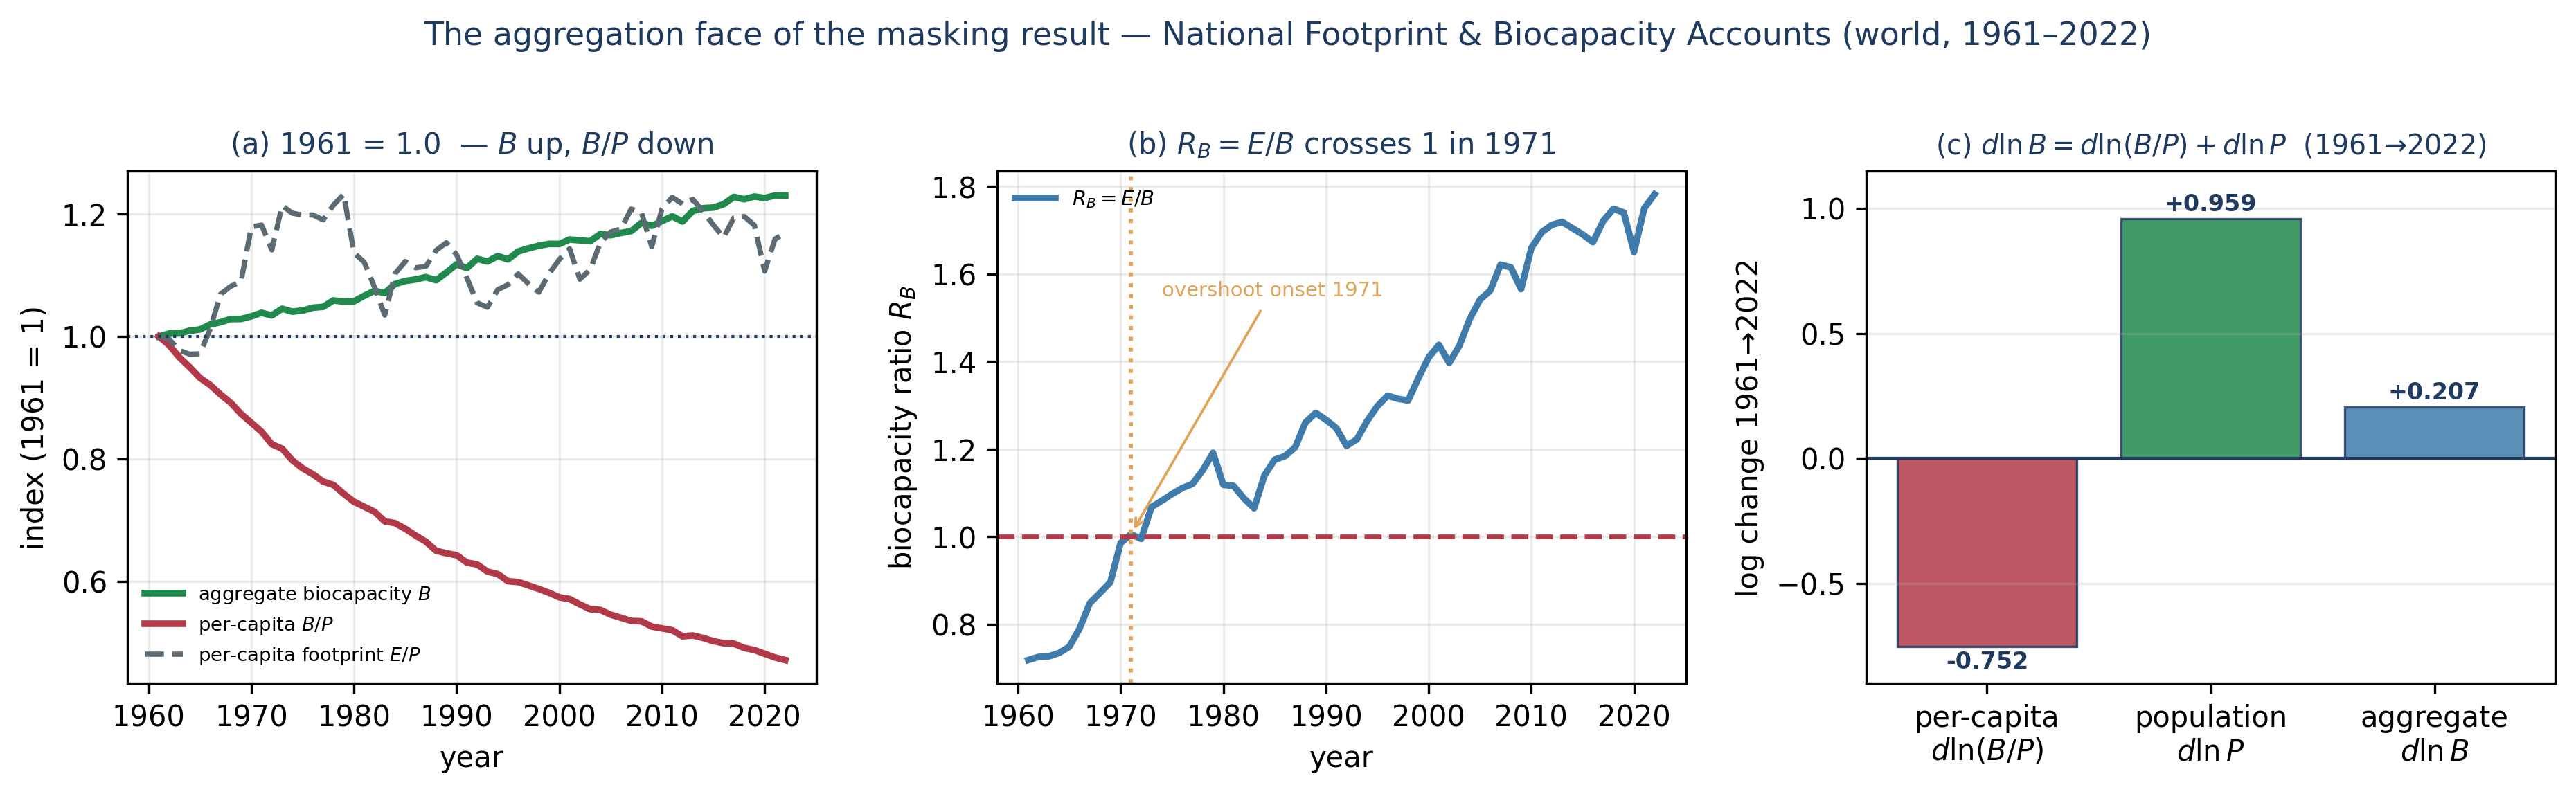
\includegraphics[width=\textwidth]{fig2_nfa_aggregation_face}
\caption{The aggregation face of the masking result, National Footprint and Biocapacity Accounts (world, 1961--2022). (a) Indices (1961 $=1$) of aggregate biocapacity $B$, per-capita biocapacity $B/P$ and per-capita footprint $E/P$: $B$ rises while $B/P$ halves. (b) The biocapacity ratio $R_B=E/B$ crosses $1$ (overshoot onset) in 1971. (c) The exact identity $d\ln B=d\ln(B/P)+d\ln P$: population $+0.959$ and per-capita $-0.752$ (shares of $\Delta\ln B$: $+464\%$ and $-364\%$). The public aggregate carries no yield/area split, so this panel is explicitly not the two-land composition mask.}
\label{fig:aggregation}
\end{figure}

To advance past the aggregate we apply the observation operator of Section~\ref{sec:data}. With $A_f$ from FAOSTAT cropland area and $b_f$ from the normalised crop-yield index calibrated at 1961, the exact Divisia decomposition \eqref{eq:divisia} attributes the $+0.207$ aggregate log-change to a yield channel $+0.393$, a cropland-area channel $+0.056$ and a residual $-0.242$ (Table~\ref{tab:divisia}). Raw component log-changes ($+1.128$, $+0.160$, $-0.404$) are changes in the components, not contributions, and cannot be summed; the log-mean weights $w_X=0.349$, $w_C=0.600$ make the identity exact, whereas average shares ($0.375$, $0.625$) would give $+0.231$. The yield channel dominates the growth of the aggregate, cropland area is a small positive, and the residual -- all biocapacity not captured by the cropland proxy -- is a large negative. The result is robust to the unidentified base-year cropland share: over $\alpha\in[0.10,0.34]$ the weighted identity sums to $+0.207$ exactly and the yield channel is the dominant positive term at every $\alpha$, although the split is not pinned ($w_X$ ranges $0.18$--$0.62$); for $\alpha\ge0.339$ the residual is no longer positive at the endpoint and the level decomposition $\Delta B=\Delta X+\Delta C$ (reproducing $\Delta B=+2.242\times10^{9}$\,gha) carries the same sign statement (SI~\S S5.2). The nominal anchor $\alpha=0.19$ can be replaced by the measured one, $b_f(1961)=B_{\mathrm{cropland,NFA}}(1961)/A_f(1961)\approx0.93\,\mathrm{gha\,ha^{-1}\,yr^{-1}}$ (cropland share $\approx0.128$), which lies inside the robustness band and leaves the decomposition unchanged. The instantaneous fast-book share $s_X$ rises from $0.19$ to $0.56$ over the period; only the growth and sign statements are robust, and $b_c$, $b_{G,c}$, $\rho_c$ and the yield/area split of the residual remain unidentified, exactly as Proposition~\ref{prop:mask}(iii) says they must.

\begin{table}[!htbp]
\centering\small
\caption{Exact log-mean (Divisia) decomposition of world aggregate biocapacity growth, 1961--2022 (NFA aggregate series; cropland proxies from FAOSTAT; base-year calibration $\alpha=0.19$). Contributions sum exactly to $\Delta\ln B=+0.207$. Raw log-changes are component changes, not contributions.}
\label{tab:divisia}
\begin{tabularx}{\textwidth}{X l l l}
\toprule
Component & Raw $\Delta\ln$ & Log-mean weight & Contribution to $\Delta\ln B$ \\
\midrule
Fast-book yield $b_f$ (crop-yield index) & $+1.128$ & $w_X=0.349$ & $+0.393$ \\
Fast-book area $A_f$ (cropland) & $+0.160$ & $w_X=0.349$ & $+0.056$ \\
Residual $C=B-b_fA_f$ (non-cropland) & $-0.404$ & $w_C=0.600$ & $-0.242$ \\
\midrule
Total & & & $+0.207$ \\
\bottomrule
\end{tabularx}
\end{table}

The measured land-type accounts make the composition explicit without any proxy (Fig.~\ref{fig:composition}). In the land-type vintage the aggregate grew $+24.5\%$ ($\Delta\ln B=+0.219$), of which cropland contributed $+23.8$ points and built-up land $+7.3$ points, while forest products, grazing land and fishing grounds together contributed $-6.6$ points; the component ratios are cropland $2.85\times$ (area $1.17\times$, per-hectare yield $2.43\times$), built-up $8.63\times$, forest products $0.90\times$, grazing $0.98\times$, fishing $0.96\times$. Cropland accounts for essentially all of the net aggregate growth ($\approx97$--$103\%$ depending on vintage), and the non-cropland book is flat at the endpoint ($1.008\times$; intra-period index up to $1.024\times$). The identifiability limit is recursive: the near-flat non-cropland total is itself the net of declining forest-products, grazing and fishing biocapacity (together $\approx-6.4\times10^{8}$\,gha) and an $8.6\times$ rise in built-up land. These categories are accounting flows and land classes rather than the model's capital stock, so the accounts do not demonstrate a measured decline in $A_c$; they do demonstrate that aggregate summary statistics conceal composition at more than one level.

\begin{figure}[!htbp]
\centering
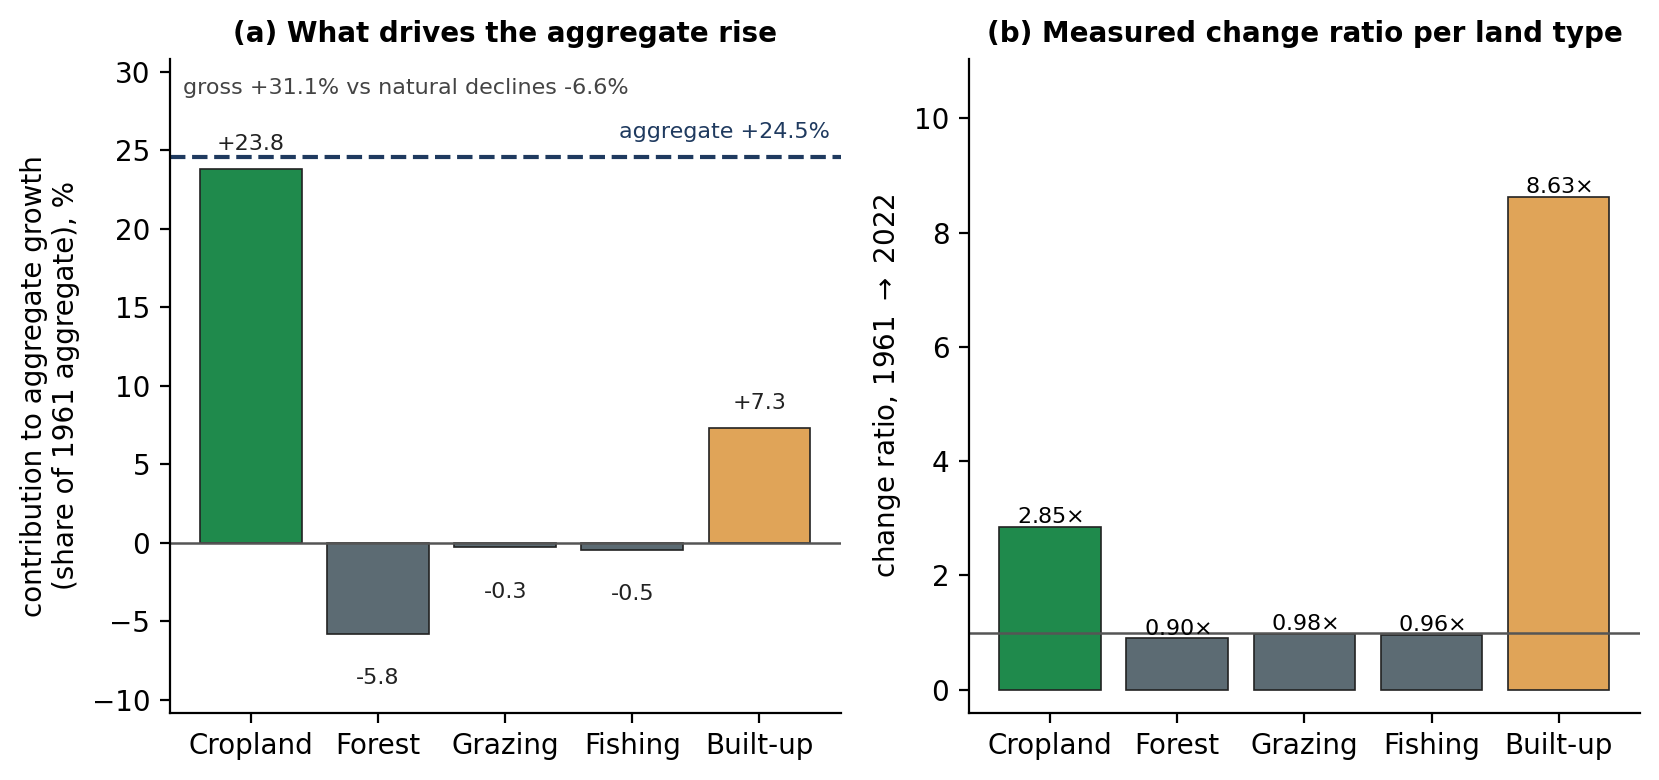
\includegraphics[width=0.95\textwidth]{fig3_composition_attribution}
\caption{Measured land-type composition of aggregate biocapacity change, National Footprint and Biocapacity Accounts (world, 1961--2022, land-type vintage). (a) Contributions to the $+24.5\%$ aggregate growth ($\Delta\ln B=+0.219$): cropland $+23.8$ points and built-up land $+7.3$ points (gross $+31.1$), against forest products, grazing and fishing $-6.6$ points; the components sum exactly to the aggregate. (b) Endpoint ratios: cropland $2.85\times$, built-up $8.63\times$, forest products $0.90\times$, grazing $0.98\times$, fishing $0.96\times$. A single aggregate number cannot reveal this composition.}
\label{fig:composition}
\end{figure}

\subsection{Falsifiable predictions}\label{sec:predictions}

The model's testable content, framed against two-book series ($B$, $A_c$, $A_f$ and land-cover/yield proxies) rather than the aggregate, is the following.
\begin{enumerate}[label=P\arabic*.,leftmargin=2.2em]
\item \textbf{Mask signature.} During conversion $\dot A_c<0$ while $\dot B\ge0$, and $R_B\le1$ is not required: the capital book can fall while the aggregate is at or below demand. Observing $\dot A_c<0$ with a steady or rising $B$ (composition mask) versus a steady $E$ (liquidation mask) discriminates the two readings (Proposition~\ref{prop:mask}).
\item \textbf{Window scale.} The duration of the mask is set by the slow eigenvalue $\lambda_1$ (through $\tconv$, $\mu$, $\eta_f$, $b_c/b_f$) and its amplitude by $\dconv$ and the deficit, not by a fixed horizon; the bulk of conversion precedes the closing of the deficit by one to two e-folding times.
\item \textbf{No critical-slowing precursor.} The return time does not grow as demand approaches the ceiling, and the drawdown depth is continuous in demand (Fig.~\ref{fig:model}c); the observable warning is the capital book approaching its typed floor (Proposition~\ref{prop:ceiling}). This is a negative prediction: a catastrophic-shift early-warning indicator is not expected to precede the two-land drawdown.
\item \textbf{Demand threshold, not delay threshold.} The initial demand that drives the capital book to its floor rises with initial capital (Table~\ref{tab:model}b) and is insensitive to the regeneration delay (identical to $10^{-3}$ for $\tau_g=5$--$40$\,yr), because the regenerative share of capital value is small and quality is monotone; a one-stock regeneration cliff is not expected.
\item \textbf{Recovery requires a gated flow.} Reducing demand does not restore the capital book; recovery requires an explicit restoration flow whose gate sign determines whether it is inert during the shortfall (surplus-gated; thresholds unchanged by $\chi_r$) or deepens it (deficit-gated).
\end{enumerate}
The identifiability statement of Proposition~\ref{prop:mask}(iii) is not a prediction but a constraint on testing: P1--P5 can be tested only with independent $A_c$ and $b_f$ proxies, never with the aggregate alone.

\section{Discussion}\label{sec:discussion}

\subsection{What the two-land structure changes, and what it removes}

The results depart from the single-stock, single-aggregate reading of the environment that dominates the resource and sustainability literature \citep{Schaefer1954,May1973,Meadows1972,Meadows2004,WackernagelRees1996,BranderTaylor1998} in three respects, each of which is a negative result as much as a positive one. First, the aggregate can rise while the capital book falls, but only as a bounded composition effect: Proposition~\ref{prop:mask} gives the exact condition and Proposition~\ref{prop:bounded} the reason it cannot persist. Second, the capital drawdown is a demand-driven floor collision. The alternative-stable-states literature \citep{Scheffer2001} predicts that a system approaching a fold shows critical slowing down, hysteresis and a discontinuous jump; none of these is present here, and their absence is structural (Table~\ref{tab:neg}): the deficit-side dynamics are affine with constant real eigenvalues, the equilibrium leaves the admissible set through a face rather than through a bifurcation, and the drawdown depth is continuous in demand. Third, recovery is not the reverse of degradation; it requires an explicit, gated flow, and the gate sign is a design decision with phase-dependent consequences.

\begin{table}[!htbp]
\centering\small
\caption{Structural properties and negative results in the two-land model, each derived under the two-land structure rather than inherited from a one-stock comparator.}
\label{tab:neg}
\begin{tabularx}{\textwidth}{>{\raggedright\arraybackslash}p{0.27\textwidth} l X}
\toprule
Phenomenon & Present? & Status in the two-land model \\
\midrule
Capital-land catastrophic fold & No & $B_{eq}(A_c)$ is strictly monotone; the balance point is unique; the transition is a typed-floor collision at $\Eceil\approx1.138$ (Proposition~\ref{prop:ceiling}) \\
Critical slowing down & No & deficit-side dynamics are affine; $\lambda_1\approx-0.054\,\mathrm{yr}^{-1}$ is constant along the branch and does not tend to $0$ \\
Hysteresis / path dependence of the balance point & No & no second branch; irreversibility of the \emph{area} book is a different property (no return flow without $R_{rc}$, Section~\ref{sec:recovery}) \\
Discontinuous collapse in demand & No & drawdown depth is continuous and monotone in $P_0$ (Fig.~\ref{fig:model}c); thresholds are tolerance-dependent bands \\
Regeneration-delay cliff & No & floor-contact threshold identical to $10^{-3}$ for $\tau_g=5$--$40$\,yr; the regenerative share of capital value is small and $q$ is monotone \\
Sustained boom--bust cycle & No & single overshoot pulse; $q$ is monotone; $r\tau_p=0.5<\pi/2$, below the Hutchinson threshold of the delayed logistic population loop \citep{Hutchinson1948} \\
Allee-type rescue threshold in capital & No & no capital level below which recovery is impossible other than the floor itself; the lever is demand or restoration, not the lag \\
\bottomrule
\end{tabularx}
\end{table}

The negative results have a direct bearing on early-warning practice. Generic indicators of critical slowing down (rising autocorrelation and variance) are motivated by the approach to a fold \citep{Scheffer2001}. In a two-book system in which the drawdown is a boundary collision, such indicators would not be expected to fire, and their silence should not be read as safety. The informative signal is the capital book itself, which requires the two-book series.

Several quantities that circulate for models of this kind are deliberately not claimed here. The two-gain Hopf classification of which delay destabilises, the associated critical delays, and the reference eigenvalue of order $+0.6$ belong to a single-stock fast--slow reduction that we retain only as a comparator in SI~\S S7, where its equations, equilibrium family and figures are given; none of its features is carried into the two-land results. The ``18--20\,yr regeneration cliff'' of the one-stock comparator does not survive the two-land structure (Table~\ref{tab:neg}). What is structural in the two-land model is the composition logic and the identifiability limit; what is conditional on effective parameters is the sign and size of $\dconv$ and the location of the ceiling.

\subsection{Measurement implications}

The methodological result of the paper is the identifiability limit. Biocapacity in global hectares is a value-weighted scalar, not a count of the underlying assets. Given only that a portfolio's value rose by $20\%$, one cannot tell whether every holding grew a little or some made large gains while others quietly fell; the scalar gloss hides the composition. This is the generic limit of any value-weighted composite \citep{Nardo2008}, and Proposition~\ref{prop:mask}(iii) states it for biocapacity: the aggregate identifies one linear combination of the areas, and the capital-book parameters enter only through identifiable combinations. The aggregate is therefore a weak-sustainability index in the precise sense of the companion assessment work \citep{Abaee2026b}: it is the linear, perfectly substitutable member of the aggregator family (its Lemma~A), and it can satisfy an aggregate floor while the typed floor on $A_c$ is violated by exactly the amount that the fast-land yield gains against the capital loss. In that family no positive-elasticity aggregator is uniformly safe and only the typed, non-compensating one is (its Theorem~S2(ii)). Under exact-tube semantics, in which a transition is safe only if every state along it satisfies the constraints, the passage during which $A_c$ falls is itself a violation even if the endpoint recovers -- a reason to report through-time trajectories and boundary curves, not endpoint attractors.

For the National Footprint Accounts the implication is concrete. The accounts are account-based and do not capture soil erosion, deforestation, groundwater depletion or other cumulative degradation, so estimated biocapacity likely overstates the real base and the footprint understates the overshoot \citep{Wackernagel2002,Borucke2013}; critics have made the point forcefully \citep{Blomqvist2013,GiampietroSaltelli2014,Galli2016,vdBerghGrazi2015}. The present results add a different and more specific point: even an internally consistent aggregate cannot be inverted into its components. A growth headline for total biocapacity carries no information about whether cropland growth is compensating for stagnation or offsetting declines elsewhere, and the measured accounts show that this is exactly what happened in 1961--2022 (Fig.~\ref{fig:composition}). The informative assessment reports components with the total -- at minimum component endpoint ratios, log contributions, attribution shares, data vintage and endpoint sensitivity -- at every level at which an aggregate is used. Parallel observations have been made for human appropriation of net primary production and for land-management data \citep{Haberl2007,Krausmann2013,Erb2017,Carvalhais2014}: the composition of a flow aggregate, not its level, carries the sustainability information.

The empirical programme that follows is a flux reconstruction, not a curve fit. The observation operator of Section~\ref{sec:data} is a hierarchy: NFA land-type biocapacity with physical area and yield factors where obtainable; FAOSTAT area and yields as independent external proxies (used here); remote-sensing land cover and historical reconstructions for validation and extension (SI~\S S5.4). Forest area is a sentinel proxy for $A_c$, not the whole capital book; capital-land regeneration is unobserved in the accounts and would require growing-stock or net-annual-increment data. The proxies do not solve global-hectare identifiability; they make the composition mechanism an independently anchored, falsifiable statement rather than an asserted one.

\subsection{Policy operators}

Three operators follow from the typed-floor structure and are developed in SI~\S S6. Freezing conversion -- capping $A_f$ or flooring $A_c$ -- is the single operator that guarantees $A_c\ge\Acmin$; a governor that observes only the composite $B$ cannot guarantee a capital-land floor, and the failure is informational rather than dynamical. Restoration is protective only when surplus-gated, and a deficit-gated flow can deepen the shortfall it is meant to relieve; this is the protective, as opposed to mobilising, institutional signature of the delay companion \citep{Abaee2026a}. A Half-Earth reservation \citep{Wilson2016}, $E\le\sigma B$ with $\sigma<1$, succeeds without liquidation on the nominal path, but this is a nominal-path consequence until it is certified against a declared disturbance class under a preregistered retention rule, and we state it as such.

\subsection{Relation to companion work}

The accounting layer -- the closed typed-flux ledger, conservation and donor-limitation rules, depletion arithmetic and the no-non-negative-weighting aggregation obstruction -- is the object of the ledger companion \citep{Abaee2026c}, which owns the static layer, cedes delay dynamics to its companions and registers a two-pool dynamical model as an open gap; the present paper supplies that minimal dynamical realisation for the global-hectare case. The aggregation theorem that places $B$ at the weak extreme of the aggregator family is from the assessment companion \citep{Abaee2026b}, and the institutional-delay regime is from the governance companion \citep{Abaee2026a}; the delays here are ecological (regeneration, demography), not institutional. We cite, and do not re-derive, those results.

\subsection{Limitations}

The capital land is an effective class, not a single land type; the single regeneration timescale, the composition diagnostic and the ceiling are effective-parameter statements, and the full vector decomposition is cited rather than re-derived. Most parameters are representative rather than estimated; $b_c$, $b_{G,c}$ and $\rho_c$ are not identifiable from a cross-section, and the regeneration anchors bound a band rather than calibrate $\rho_c$ (the anchors concern the regeneration rate, not the lag $\tau_g$). The per-capita footprint is held constant to isolate the stock--flow--demand feedbacks; endogenising $e$ is an extension. The composition window is bounded and demand-driven; without a sustained shortfall or a technology/demand feedback it closes at the balance point. Stability at $S=0$ is one-sided because the positive part is exact. Drawdown thresholds are tolerance-dependent bands; a small margin next to that band is reported as such and not as a sharp boundary. The debt-repayment rate is set physical and non-singular ($\eta=0.05\,\mathrm{yr}^{-1}$); the $\eta\to0$ case removes the debt equilibrium and is excluded by a floor, and outcomes are insensitive to $\eta$ over a modest positive range. The accounts do not separate yield from area, which is the identifiability limitation the paper is about rather than an estimation error. Finally, the delayed-regeneration term is implemented at the current quality in the deposited solver (Section~\ref{sec:numerics}); we have verified that applying the delay changes no reported quantity by more than $1\%$, and the corrected variant is deposited alongside.

\section{Conclusions}\label{sec:conclusions}

A single aggregate of annual bioproductive supply can conceal the composition of what is growing, and the concealment is structural. In a minimal two-land model with conserved area, a separate quality state and demand-driven conversion, the aggregate rises while the ecological-capital book falls whenever the fast-land yield exceeds the per-hectare value of capital land (Proposition~\ref{prop:mask}); from the aggregate alone the capital loss is unidentified, and independent fast-book proxies identify at most a measured fast book and a residual. The drawdown of the capital book under sustained demand is a floor collision at a demand ceiling, not a catastrophic shift: the deficit-side dynamics are affine, the leading eigenvalue is constant along the branch, there is no fold, no hysteresis and no critical slowing down, and the drawdown depth is a continuous function of demand (Proposition~\ref{prop:ceiling}). The mask is bounded because technology lifts the fast yield by at most a fixed factor whereas debt erosion is limited only by the sustained shortfall (Proposition~\ref{prop:bounded}), and recovery requires an explicit restoration flow whose gate sign matters. In the measured National Footprint and Biocapacity Accounts for 1961--2022, aggregate biocapacity grew $23\%$ while per-capita biocapacity halved, the exact Divisia decomposition attributes the growth to cropland yield with a negative non-cropland residual, and the land-type accounts show cropland biocapacity growing $2.85\times$ against a flat non-cropland book that is itself the net of declining forest, grazing and fishing biocapacity and rising built-up land. These results establish an identifiability property of aggregate biocapacity and a measured composition pattern; they are not a forecast and do not show a measured decline in the model's ecological-capital stock. Their practical content is a reporting rule: an aggregate biocapacity total is informative only when its components are reported alongside it, at every level at which the aggregate is used. A modern economy can run for decades on a harvest that looks healthy while the orchard behind it quietly shrinks; the harvest number will not say so, and only the two-book series can.

\section*{Declarations}

\paragraph{Data availability} Code and data are available at \url{https://zenodo.org/records/22554480}. This study reports no new empirical dataset; the empirical inputs are published values (NFA 2025 edition, FAOSTAT) used to bound the regeneration timescale and to decompose the composition of aggregate biocapacity. The scripts that regenerate Fig.~\ref{fig:model} and Table~\ref{tab:model} from the deposited model code accompany the Supplementary Information.

\paragraph{Funding} No funding was received.

\paragraph{Competing interests} The author declares no competing interests.

\paragraph{CRediT authorship contribution statement} \textbf{Amin Abaee:} Conceptualization; Methodology; Software; Formal analysis; Writing -- original draft; Writing -- review \& editing.

\paragraph{Declaration of generative AI in scientific writing} DeepSeek AI and Claude (Anthropic) assisted with computational-reproducibility checks and language editing under the author's supervision; the author reviewed and edited the content and takes full responsibility for the publication.

\begin{thebibliography}{99}
\bibitem[{Abaee(2026a)}]{Abaee2026a} Abaee, A. (2026a). \emph{Governance delay and the stability of harvested stocks: mobilising and protective feedback rules, and the review interval as a design parameter.} Zenodo. \url{https://doi.org/10.5281/zenodo.22554217}.
\bibitem[{Abaee(2026b)}]{Abaee2026b} Abaee, A. (2026b). \emph{Aggregate Indices and Transition Safety: A Quantifier-Order Separation Between Scalarized and Coordinate-Wise Feasibility.} Zenodo. \url{https://doi.org/10.5281/zenodo.22545740}.
\bibitem[{Abaee(2026c)}]{Abaee2026c} Abaee, A. (2026c). \emph{Typed Flux Ledgers and Depletion Arithmetic: Conservation, Componentwise Diagnostics, and the Semantics of Depletion Horizons.} Zenodo. \url{https://doi.org/10.5281/zenodo.22554177}.
\bibitem[{Anderies(2000)}]{Anderies2000} Anderies, J. M. (2000). On modeling human behavior and institutions in simple ecological economic systems. \emph{Ecological Economics}, 35(3), 393--412.
\bibitem[{Becker et al.(2017)}]{Becker2017} Becker, W., Saisana, M., Paruolo, P. \& Vandecasteele, I. (2017). Weights and importance in composite indicators: Closing the gap. \emph{Ecological Indicators}, 80, 12--22.
\bibitem[{Blomqvist et al.(2013)}]{Blomqvist2013} Blomqvist, L., Brook, B. W., Ellis, E. C., Kareiva, P. M., Nordhaus, T. \& Shellenberger, M. (2013). Does the shoe fit? Real versus imagined ecological footprints. \emph{PLoS Biology}, 11(11), e1001700.
\bibitem[{Borucke et al.(2013)}]{Borucke2013} Borucke, M., Moore, D., Cranston, G., Gracey, K., Iha, K., Larson, J., Lazarus, E., Morales, J. C., Wackernagel, M. \& Galli, A. (2013). Accounting for demand and supply of the biosphere's regenerative capacity: The National Footprint Accounts' underlying methodology and framework. \emph{Ecological Indicators}, 24, 518--533.
\bibitem[{Brander and Taylor(1998)}]{BranderTaylor1998} Brander, J. A. \& Taylor, M. S. (1998). The simple economics of Easter Island: A Ricardo--Malthus model of renewable resource use. \emph{American Economic Review}, 88(1), 119--138.
\bibitem[{Calvin and Bond-Lamberty(2018)}]{CalvinBondLamberty2018} Calvin, K. \& Bond-Lamberty, B. (2018). Integrated human--Earth system modeling --- state of the science and future directions. \emph{Environmental Research Letters}, 13(6), 063006.
\bibitem[{Carvalhais et al.(2014)}]{Carvalhais2014} Carvalhais, N., Forkel, M., Khomik, M., Bellarby, J., Jung, M., Migliavacca, M., Mu, M., Saatchi, S., Santoro, M., Thurner, M., Weber, U., Ahrens, B., Beer, C., Cescatti, A., Randerson, J. T. \& Reichstein, M. (2014). Global covariation of carbon turnover times with climate in terrestrial ecosystems. \emph{Nature}, 514(7521), 213--217.
\bibitem[{Cohen(1995)}]{Cohen1995} Cohen, J. E. (1995). Population growth and Earth's human carrying capacity. \emph{Science}, 269(5222), 341--346.
\bibitem[{Copernicus(2019)}]{Copernicus2019} Copernicus (2019). \emph{Global Land Cover LC100.} European Commission, Land Copernicus.
\bibitem[{Dasgupta(2021)}]{Dasgupta2021} Dasgupta, P. (2021). \emph{The Economics of Biodiversity: The Dasgupta Review.} London: HM Treasury.
\bibitem[{Diamond(2005)}]{Diamond2005} Diamond, J. (2005). \emph{Collapse: How Societies Choose to Fail or Succeed.} New York: Viking.
\bibitem[{Donges et al.(2017)}]{Donges2017} Donges, J. F., Winkelmann, R., Cornell, S. E., Lucht, W., Dyke, J. G., Rockstr\"om, J., Heitzig, J. \& Schellnhuber, H. J. (2017). Closing the loop: Reconnecting human dynamics to Earth system science. \emph{The Anthropocene Review}, 4(2), 151--157.
\bibitem[{Erb et al.(2017)}]{Erb2017} Erb, K.-H., Luyssaert, S., Meyfroidt, P., Pongratz, J., Don, A., Kloster, S., Kuemmerle, T., Fetzel, T., Fuchs, R., Hasegawa, T., Haberl, H., et al. (2017). Land management: data availability and process understanding for global change studies. \emph{Global Change Biology}, 23(2), 512--533.
\bibitem[{ESA(2017)}]{ESA2017} ESA (2017). \emph{Land Cover CCI Product User Guide, Version 2.0.} European Space Agency.
\bibitem[{FAO(2020)}]{FAO2020} FAO (2020). \emph{Global Forest Resources Assessment 2020: Main Report.} Rome: Food and Agriculture Organization.
\bibitem[{FAO(2023)}]{FAO2023} FAO (2023). \emph{FAOSTAT: Land Use; Crops and Livestock Products.} Rome: Food and Agriculture Organization.
\bibitem[{Fischer et al.(2022)}]{Fischer2022} Fischer, S. M., Joy, M. K., Abrahamse, W., Milfont, T. L. \& Petherick, L. M. (2022). The use and misuse of composite environmental indices. \emph{bioRxiv}, 2022.03.15.484501. \url{https://doi.org/10.1101/2022.03.15.484501}.
\bibitem[{Galli et al.(2016)}]{Galli2016} Galli, A., Giampietro, M., Goldfinger, S., Lazarus, E., Lin, D., Saltelli, A., Wackernagel, M. \& M\"uller, F. (2016). Questioning the ecological footprint. \emph{Ecological Indicators}, 69, 224--232.
\bibitem[{Giampietro and Saltelli(2014)}]{GiampietroSaltelli2014} Giampietro, M. \& Saltelli, A. (2014). Footprints to nowhere. \emph{Ecological Indicators}, 46, 610--621.
\bibitem[{Haberl et al.(2007)}]{Haberl2007} Haberl, H., Erb, K.-H., Krausmann, F., Gaube, V., Bondeau, A., Plutzar, C., Gingrich, S., Lucht, W. \& Fischer-Kowalski, M. (2007). Quantifying and mapping the human appropriation of net primary production in earth's terrestrial ecosystems. \emph{PNAS}, 104(31), 12942--12947.
\bibitem[{Henderson and Loreau(2018)}]{HendersonLoreau2018} Henderson, K. \& Loreau, M. (2018). How ecological feedbacks between human population and land cover influence sustainability. \emph{PLoS Computational Biology}, 14(8), e1006389.
\bibitem[{Hurtt et al.(2011)}]{Hurtt2011} Hurtt, G. C., Chini, L. P., Frolking, S., Betts, R. A., Feddema, J., Fischer, G., et al. (2011). Harmonization of land-use scenarios for the period 1500--2100: 600 years of global gridded annual land-use transitions, wood harvest, and resulting secondary lands. \emph{Climatic Change}, 109(1--2), 117--161.
\bibitem[{Hutchings and Reynolds(2004)}]{HutchingsReynolds2004} Hutchings, J. A. \& Reynolds, J. D. (2004). Marine fish population collapses: consequences for recovery and extinction risk. \emph{BioScience}, 54(4), 297--309.
\bibitem[{Hutchinson(1948)}]{Hutchinson1948} Hutchinson, G. E. (1948). Circular causal systems in ecology. \emph{Annals of the New York Academy of Sciences}, 50(4), 221--246.
\bibitem[{Klein Goldewijk et al.(2017)}]{KleinGoldewijk2017} Klein Goldewijk, K., Beusen, A., Doelman, J. \& Stehfest, E. (2017). Anthropogenic land use estimates for the last 12,000 years --- HYDE 3.2. \emph{Earth System Science Data}, 9(2), 927--953.
\bibitem[{Krausmann et al.(2013)}]{Krausmann2013} Krausmann, F., Erb, K.-H., Gingrich, S., Haberl, H., Bondeau, A., Gaube, V., Lauk, C., Plutzar, C. \& Searchinger, T. D. (2013). Global human appropriation of net primary production doubled in the 20th century. \emph{PNAS}, 110(25), 10324--10329.
\bibitem[{Kuang(1993)}]{Kuang1993} Kuang, Y. (1993). \emph{Delay Differential Equations, with Applications in Population Dynamics.} Academic Press.
\bibitem[{Lin et al.(2018)}]{Lin2018} Lin, D., Hanscom, L., Murthy, A., Galli, A., Evans, M., Neill, E., et al. (2018). Ecological footprint accounting for countries: updates and results of the National Footprint Accounts. \emph{Sustainability}, 10(12).
\bibitem[{May(1973)}]{May1973} May, R. M. (1973). \emph{Stability and Complexity in Model Ecosystems.} Princeton: Princeton University Press.
\bibitem[{Meadows et al.(1972)}]{Meadows1972} Meadows, D. H., Meadows, D. L., Randers, J. \& Behrens, W. W. (1972). \emph{The Limits to Growth.} New York: Universe Books.
\bibitem[{Meadows et al.(2004)}]{Meadows2004} Meadows, D. H., Randers, J. \& Meadows, D. L. (2004). \emph{The Limits to Growth: The 30-Year Update.} White River Junction, VT: Chelsea Green.
\bibitem[{Meadows et al.(1974)}]{Meadows1974} Meadows, D. L., Behrens, W. W., Meadows, D. H., Naill, R. F., Randers, J. \& Zahn, E. (1974). \emph{Dynamics of Growth in a Finite World.} Cambridge, MA: Wright-Allen Press.
\bibitem[{Meyer(1994)}]{Meyer1994} Meyer, P. S. (1994). Bi-logistic growth. \emph{Technological Forecasting and Social Change}, 47(1), 89--102.
\bibitem[{Meyer and Ausubel(1999)}]{MeyerAusubel1999} Meyer, P. S. \& Ausubel, J. H. (1999). Carrying capacity: A model with logistically varying limits. \emph{Technological Forecasting and Social Change}, 61(3), 209--214.
\bibitem[{Monfreda et al.(2008)}]{Monfreda2008} Monfreda, C., Ramankutty, N. \& Foley, J. A. (2008). Farming the planet: 2. Geographic distribution of crop areas, yields, physiological types, and net primary production in the year 2000. \emph{Global Biogeochemical Cycles}, 22(1), GB1022.
\bibitem[{Motesharrei et al.(2016)}]{Motesharrei2016} Motesharrei, S., Rivas, J., Kalnay, E., Asrar, G. R., Busalacchi, A. J., Cahalan, R. F., Cane, M. A., Colwell, R. R., Feng, K., Franklin, R. S., et al. (2016). Modeling sustainability: Population, inequality, consumption, and bidirectional coupling of the Earth and human systems. \emph{National Science Review}, 3(4), 470--494.
\bibitem[{Nardo et al.(2008)}]{Nardo2008} Nardo, M., Saisana, M., Saltelli, A., Tarantola, S., Hoffmann, A. \& Giovannini, E. (2008). \emph{Handbook on Constructing Composite Indicators: Methodology and User Guide.} Paris: OECD Publishing.
\bibitem[{Neubauer et al.(2013)}]{Neubauer2013} Neubauer, P., Jensen, O. P., Hutchings, J. A. \& Baum, J. K. (2013). Resilience and recovery of overexploited marine populations. \emph{Science}, 340(6130), 347--349.
\bibitem[{Pearl(1925)}]{Pearl1925} Pearl, R. (1925). \emph{The Biology of Population Growth.} New York: Alfred A. Knopf.
\bibitem[{Poeplau et al.(2011)}]{Poeplau2011} Poeplau, C., et al. (2011). Temporal dynamics of soil organic carbon after land-use change. \emph{Global Change Biology}, 17(7), 2415--2427.
\bibitem[{Poorter et al.(2016)}]{Poorter2016} Poorter, L., et al. (2016). Biomass resilience of Neotropical secondary forests. \emph{Nature}, 530(7590), 211--214.
\bibitem[{Schaefer(1954)}]{Schaefer1954} Schaefer, M. B. (1954). Some aspects of the dynamics of populations important to the management of the commercial marine fisheries. \emph{Bulletin of the Inter-American Tropical Tuna Commission}, 1(2), 25--56.
\bibitem[{Scheffer et al.(2001)}]{Scheffer2001} Scheffer, M., Carpenter, S., Foley, J. A., Folke, C. \& Walker, B. (2001). Catastrophic shifts in ecosystems. \emph{Nature}, 413(6856), 591--596.
\bibitem[{Simon(1996)}]{Simon1996} Simon, J. L. (1996). \emph{The Ultimate Resource 2.} Princeton: Princeton University Press.
\bibitem[{Tainter(1988)}]{Tainter1988} Tainter, J. A. (1988). \emph{The Collapse of Complex Societies.} Cambridge: Cambridge University Press.
\bibitem[{United Nations(2022)}]{UN2022} United Nations (2022). \emph{World Population Prospects 2022: Summary of Results.} New York: Department of Economic and Social Affairs, Population Division.
\bibitem[{van den Bergh and Grazi(2015)}]{vdBerghGrazi2015} van den Bergh, J. C. J. M. \& Grazi, F. (2015). Reply to the first systematic response by the Global Footprint Network to criticism: a real debate finally? \emph{Ecological Indicators}, 58, 458--463.
\bibitem[{van den Bergh and Rietveld(2004)}]{vdBerghRietveld2004} van den Bergh, J. C. J. M. \& Rietveld, P. (2004). Reconsidering the limits to world population: Meta-analysis and meta-prediction. \emph{BioScience}, 54(3), 195--204.
\bibitem[{Wackernagel and Rees(1996)}]{WackernagelRees1996} Wackernagel, M. \& Rees, W. (1996). \emph{Our Ecological Footprint: Reducing Human Impact on the Earth.} New Society Publishers.
\bibitem[{Wackernagel et al.(2002)}]{Wackernagel2002} Wackernagel, M., et al. (2002). Tracking the ecological overshoot of the human economy. \emph{PNAS}, 99(14), 9266--9271.
\bibitem[{Wilson(2016)}]{Wilson2016} Wilson, E. O. (2016). \emph{Half-Earth: Our Planet's Fight for Life.} New York: Liveright.
\end{thebibliography}

\end{document}
